\problemname{Looking for Waldo}

You may know the game \emph{Where is Waldo?}.
In this game you need to find a person named Waldo in a crowd of people.
This problem is kind of similar.
You need to find an axis-aligned rectangle of minimal area which contains the letters \texttt{W}, \texttt{A}, \texttt{L}, \texttt{D} and \texttt{O} and those letters are hidden in a crowd of other letters.

\begin{figure}[!h]
  \centering
  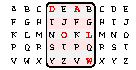
\includegraphics[width=0.5\textwidth]{sample2}
  \caption{Illustration of the second sample case.}
\end{figure}

\section*{Input}
The input consists of:
\begin{itemize}
	\item One line with two integers $h$ and $w$ $(1\leq h, w \leq 10^5$, $h\cdot{}w \leq 10^5)$, the height and width of the grid of letters.
  \item $h$ lines, each with $w$ upper case letters \texttt{A}-\texttt{Z}, the grid of letters.
\end{itemize}

\section*{Output}
Output the area of the smallest axis-aligned rectangle which contains at least one of each of the letters \texttt{W}, \texttt{A}, \texttt{L}, \texttt{D} and \texttt{O}.
If there is no rectangle containing those letters, output \texttt{impossible}.
